\documentclass[a4paper]{article}
\usepackage{array}  
\usepackage{graphicx}
\graphicspath{ {./images/} }
\usepackage[table]{xcolor}% http://ctan.org/pkg/xcolor
\usepackage{geometry}
\geometry{margin=1.25in}
\usepackage{hhline}
\usepackage{environ}
\usepackage{longtable}
 %\geometry{
 %a4paper,z
 %total={170mm,257mm},
 %left=40mm,
 %right=40mm
 %}
 \newcommand{\colWidth}{141mm}

\begin{document} 
\section*{Demo day: \textit{(Demo 1)} Group \textit{(11 - FE.ED)}}

% ------------GOALS----------

\begin{center}
\begin{tabular}{|p{\colWidth}|}
	\hline
	\cellcolor{blue!25}\large
	\textbf{What were your goals?}
	\\ \hline
	\vtop to 90mm{
As discussed in the project plan, we split our goals into 3 main areas; Robotics, Server and App. Our goals across these areas were as follows : \par
\vspace{2mm}
Robotics
\begin{itemize}
    \item Robot can dispense food into a bowl 
    \begin{itemize}
        \item One hatch will open to dispense food from the food container into the weighing chamber
        \item The weighing chamber will then open and the food will be dispensed into a chute which leads into a bowl

    \end{itemize}
\end{itemize}

Server
\begin{itemize}
    \item Server has user authentication
    \begin{itemize}
        \item Makes sure that only authorised users have access to the app and the robot 
        \begin{itemize}
            \item users must register an account before being able to sign in
        \end{itemize}
            

        \item Server can send and receive messages from the app and the robot
        \begin{itemize}
            \item Allows the app and the robot to communicate through the server
        \end{itemize}
    \end{itemize}
        
\end{itemize}

App
\begin{itemize}
    \item App has homepage, login and sign up pages 
    \begin{itemize}
        \item Allows pet owners to create an account and sign in so they can use the robot
    \end{itemize}
\end{itemize}
  }
  \\
  \hline
\end{tabular}
\vskip 5mm

% ------------ORGANISATION----------

\begin{tabular}{|p{\colWidth}|}
	\hline
	\cellcolor{blue!25}\large
	\textbf{Summarise how your group organised the workload to achieve your goals.}
	\\ \hline
	\vtop to 40mm{
We separated into sub-teams in order to work efficiently to achieve our goals. Across the project, we had 4 people working on robotics, 2 people working on the app, and 2 people working on the server. To ensure that the overall project was cohesive, the project manager worked between sub-teams to ensure that everything was running to plan and any important issues were clearly communicated. These were also brought up at weekly team meetings and discussed.
  }
  \\
  \hline
\end{tabular}
\vskip 5mm

% ------------ACHIEVEMENTS----------

\begin{tabular}{|p{\colWidth}|}
	\hline
	\cellcolor{blue!25}\large
	\textbf{What were your main achievements?}
	\\ \hline
	\vtop to 50mm{
Our main achievements were setting up the user authentication on the server. We also created forms for registering and logging in which are responsive, which then goes to a homepage when the user is authenticated or registered. Another significant achievement was developing a robust design of our prototype, although this may be altered in the future, this is because for future demos we need to make sure that our design is extendable for our additional features, such as needing to make the slide move to allow the slide to put food into different bowls.
  }
  \\
  \hline
\end{tabular}
\vskip 5mm

% ------------NOT ACHIEVED----------

\begin{tabular}{|p{\colWidth}|}
	\hline
	\cellcolor{blue!25}\large
	\textbf{What did you not achieve? Briefly explain why.}
	\\ \hline
	\vtop to 50mm{
We were not able to achieve having hatches that can open and close on the food containers. This is because we may need to 3D print the containers in order to make sure they are the right shape and size. Moreover, we have not finalised the specific design of our robot, so we did not want to commit to 3D printing anything as it may become redundant later. 
  }
  \\
  \hline
\end{tabular}
\vskip 5mm

% ------------QUANTITIVE----------

\begin{tabular}{|p{\colWidth}|}
	\hline
	\cellcolor{blue!25}\large
	\textbf{Include any quantitative data you have collected (this can be a graph/table with a few words)}
	\\ \hline
	\vtop to 200mm{
Analysis for the robot (20 times): This to see the success of the weighing chamber dropping food on to the slide, below are the results:
\begin{itemize}
    \item Complete Success (CS) - all food the in chamber was dispensed with no problems
    \item Partial Success (PS) - the majority of the food in the chamber (over $60\%$) was dispensed with no problems
    \item Partial Failure (PF) -  A significant proportion of food in the chamber was not dispensed (over $60\%$)
    \item Complete Failure (CF) - There was a significant issue with the robot (a part broke or the motor did not run)
    \end{itemize}
    

\begin{center}
\begin{tabular}{||C| C| C| C||}
\hline \hline
 CS & PS & PF & CF \\ \hline
7 & 8  & 5  & 0    \\
\hline \hline
                    
\end{tabular}
    
\end{center}


Analysis for app registering (15 times):

This is to see the success of registering a user and logging in. We registered 15 random users and also logged them in. This was $100\%$ successful.


  }
  \\
  \hline
\end{tabular}
\vskip 5mm


\begin{tabular}{|p{\colWidth}|}
	\hline
	\cellcolor{blue!25}\large
	\textbf{Include any quantitative data you have collected (this can be a graph/table with a few words)}
	\\ \hline
	\vtop to 200mm{
	\vspace{2mm}
	
	Responsiveness of the app:
As  it is a web app, responsiveness is something important for user interaction, therefore as part of our quantitative analysis we decided to visualise what our app looked like on phones, tablets and laptops with different rotational looks . \par

Laptop Screens: 

 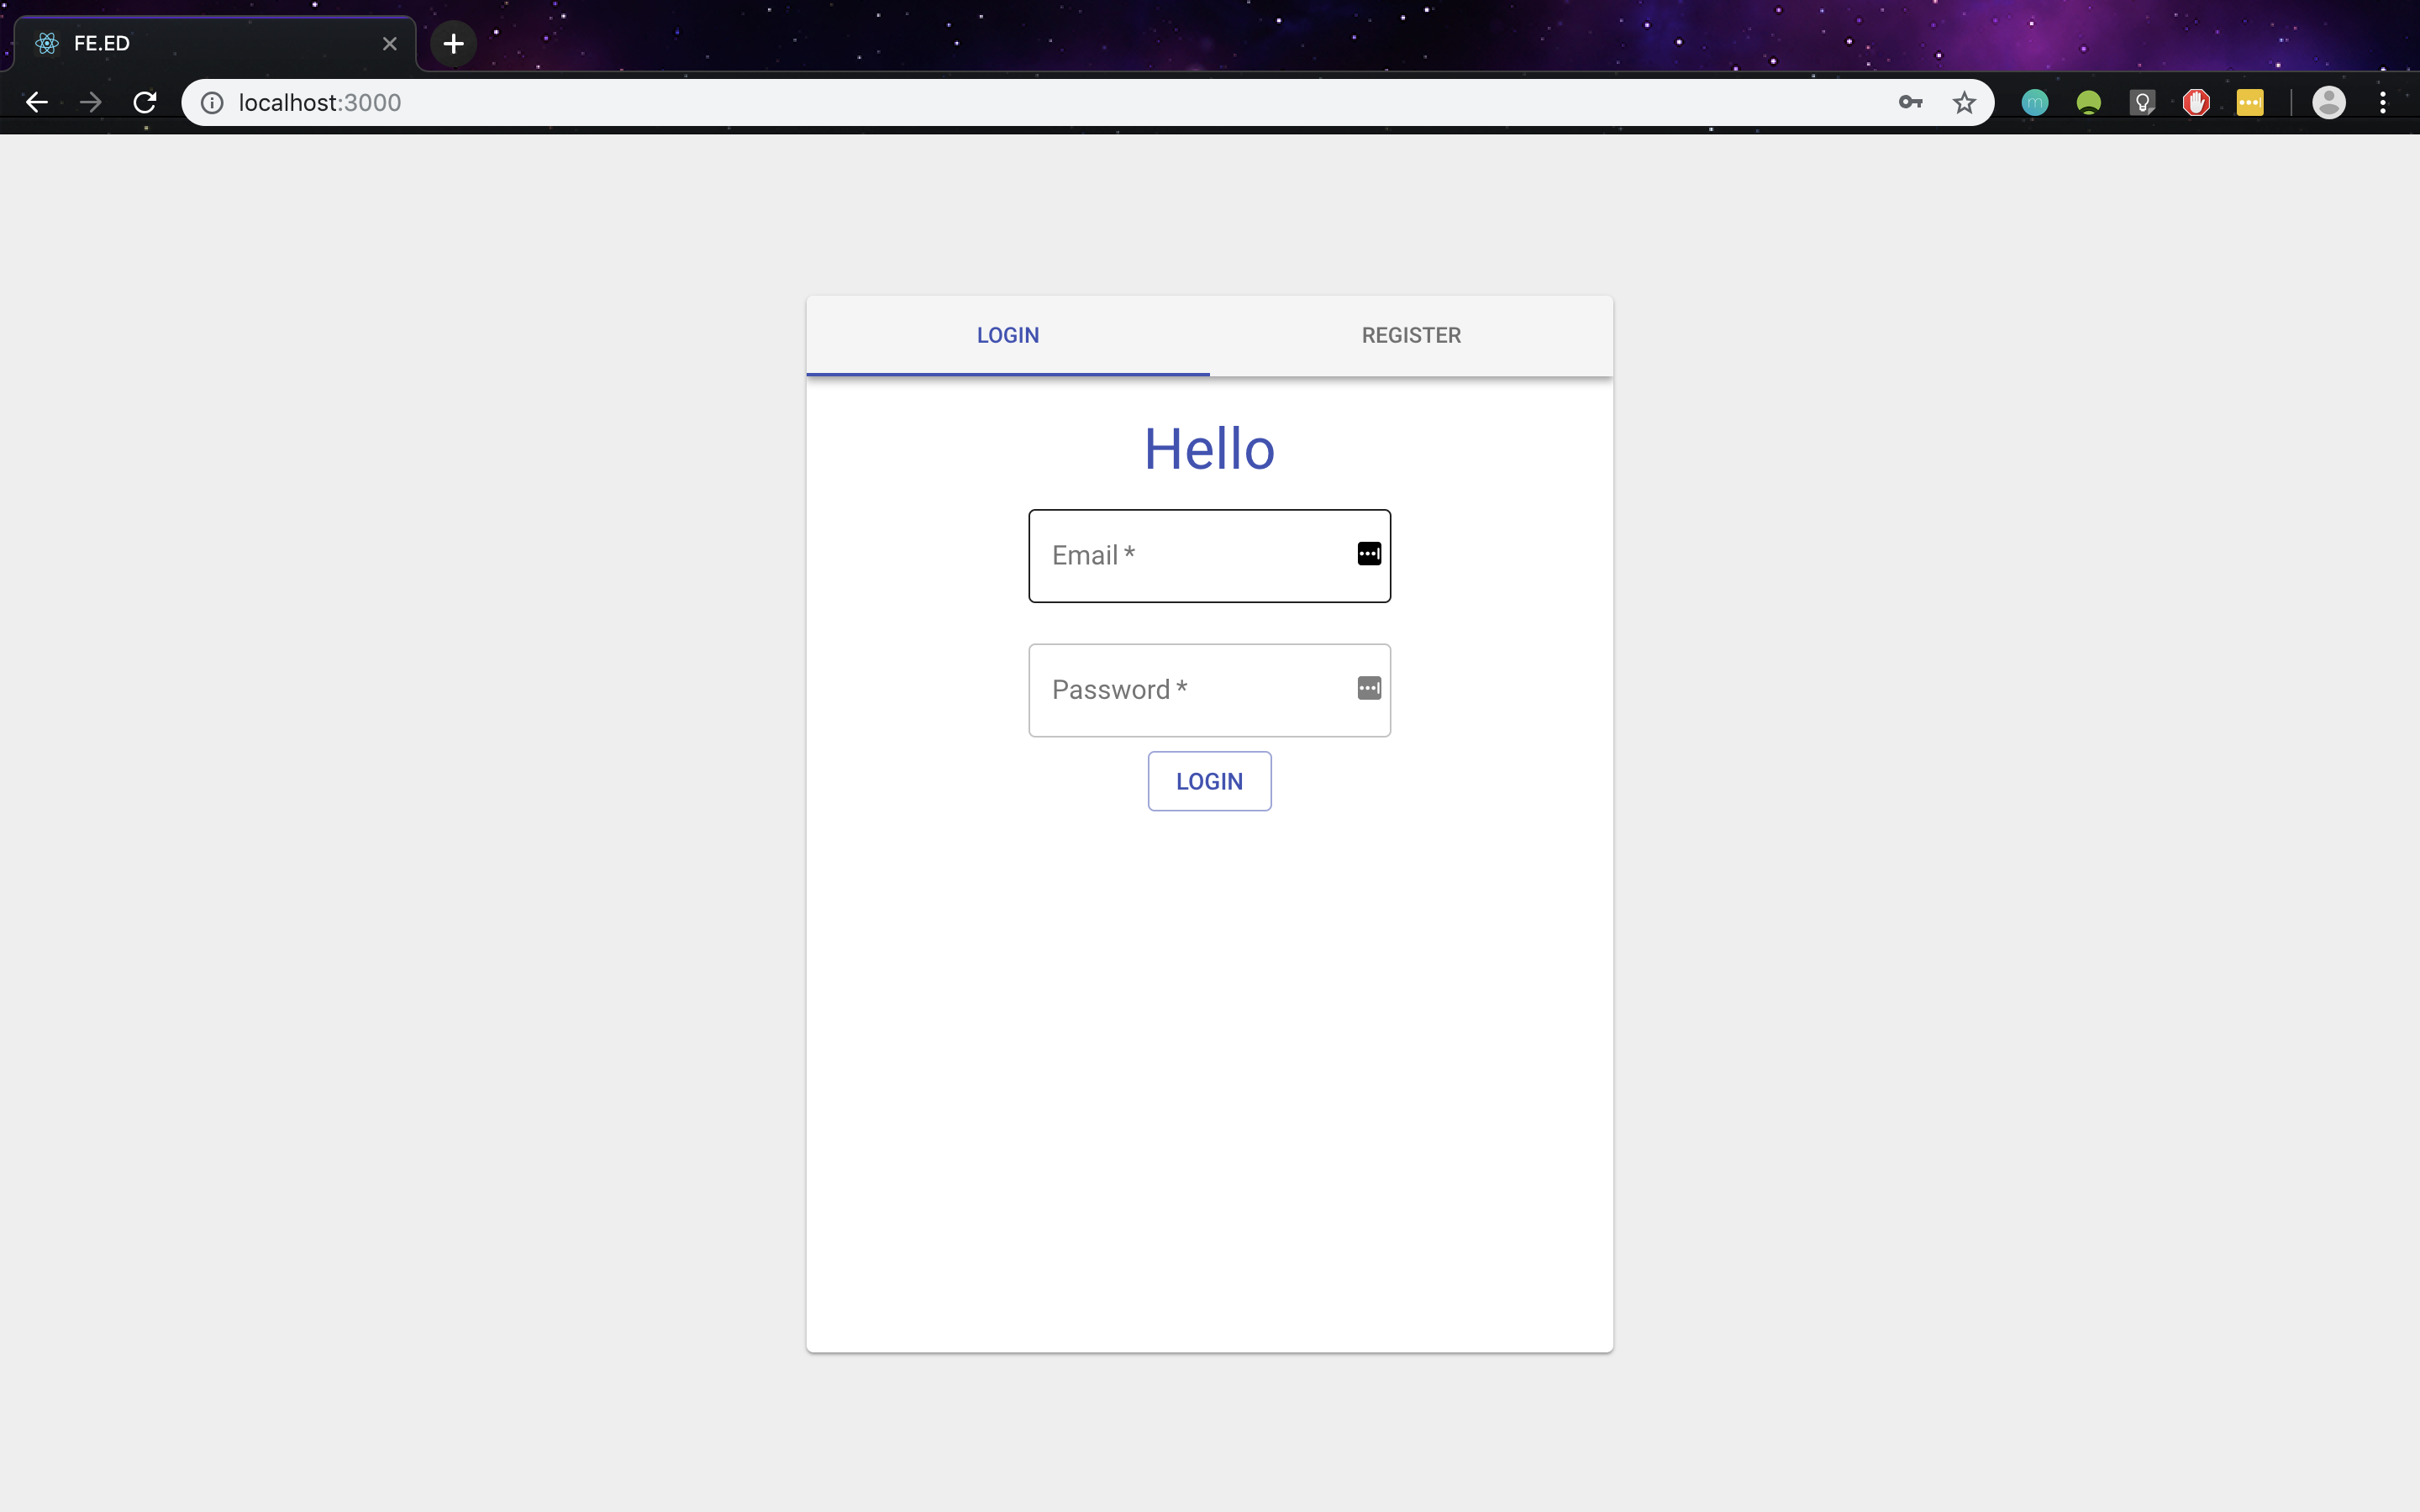
\includegraphics[width=6cm]{laptop_login.png}
 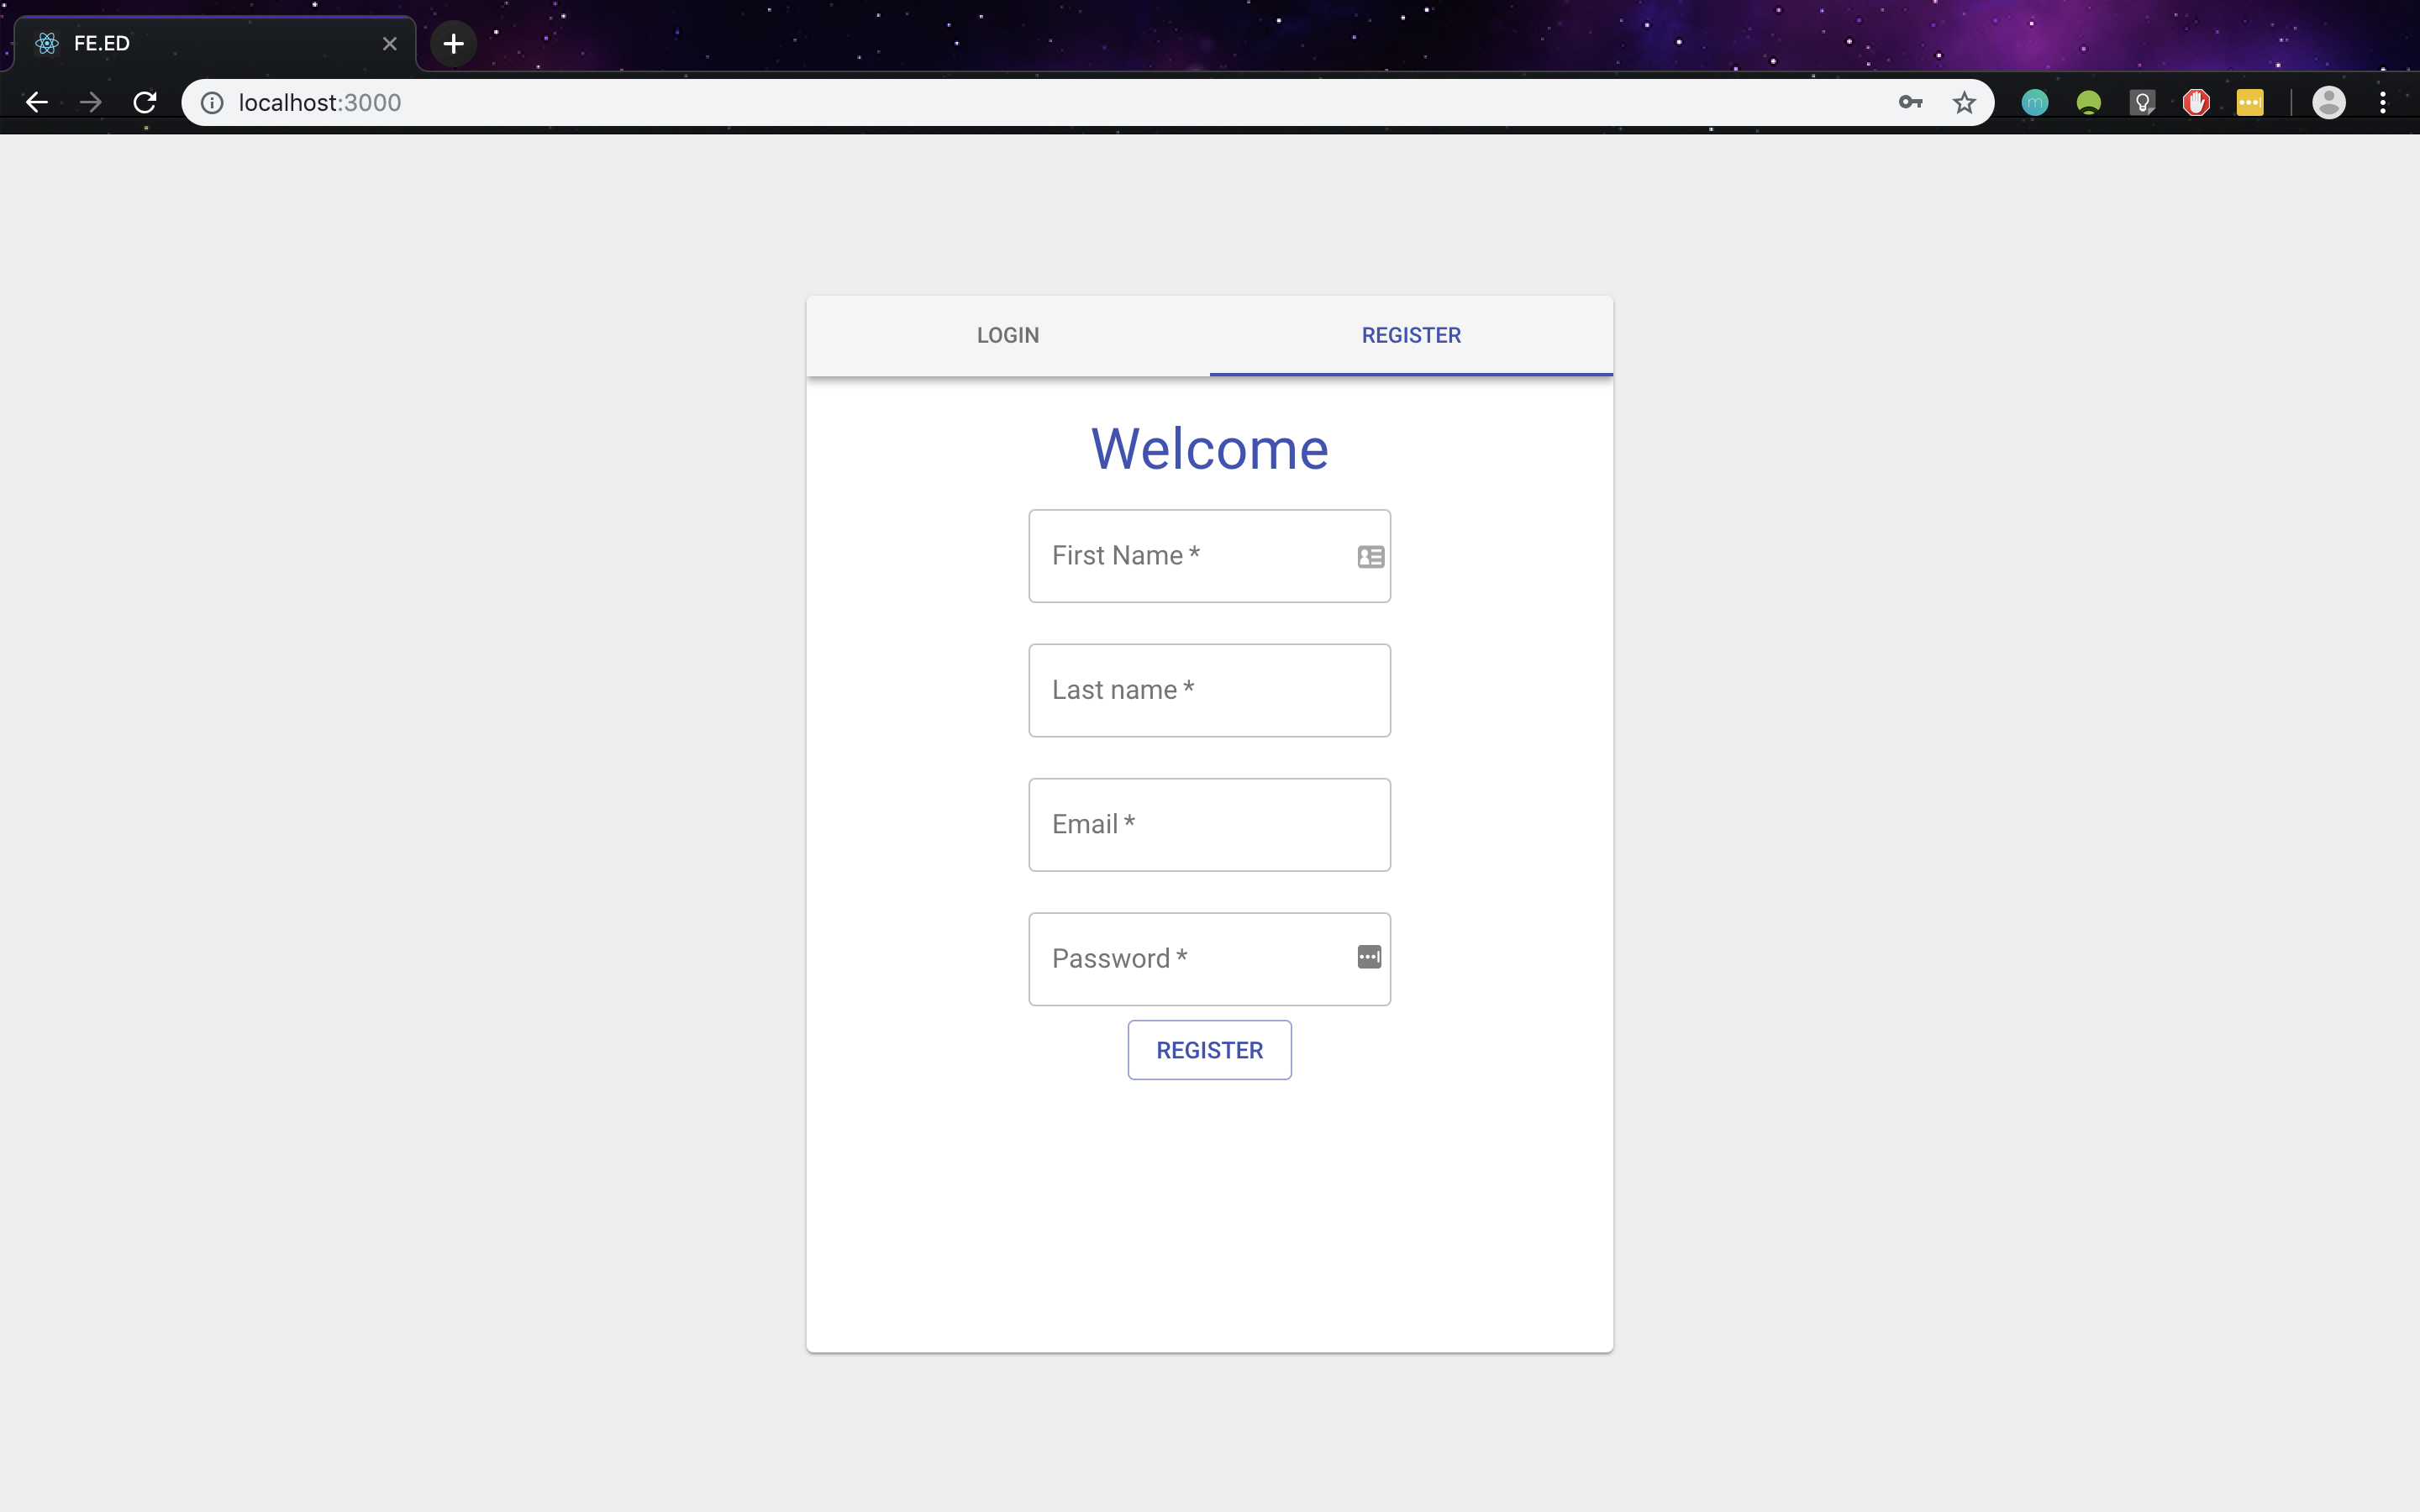
\includegraphics[width=6cm]{laptop_register.png}
 
 Tablet vertical:
 
 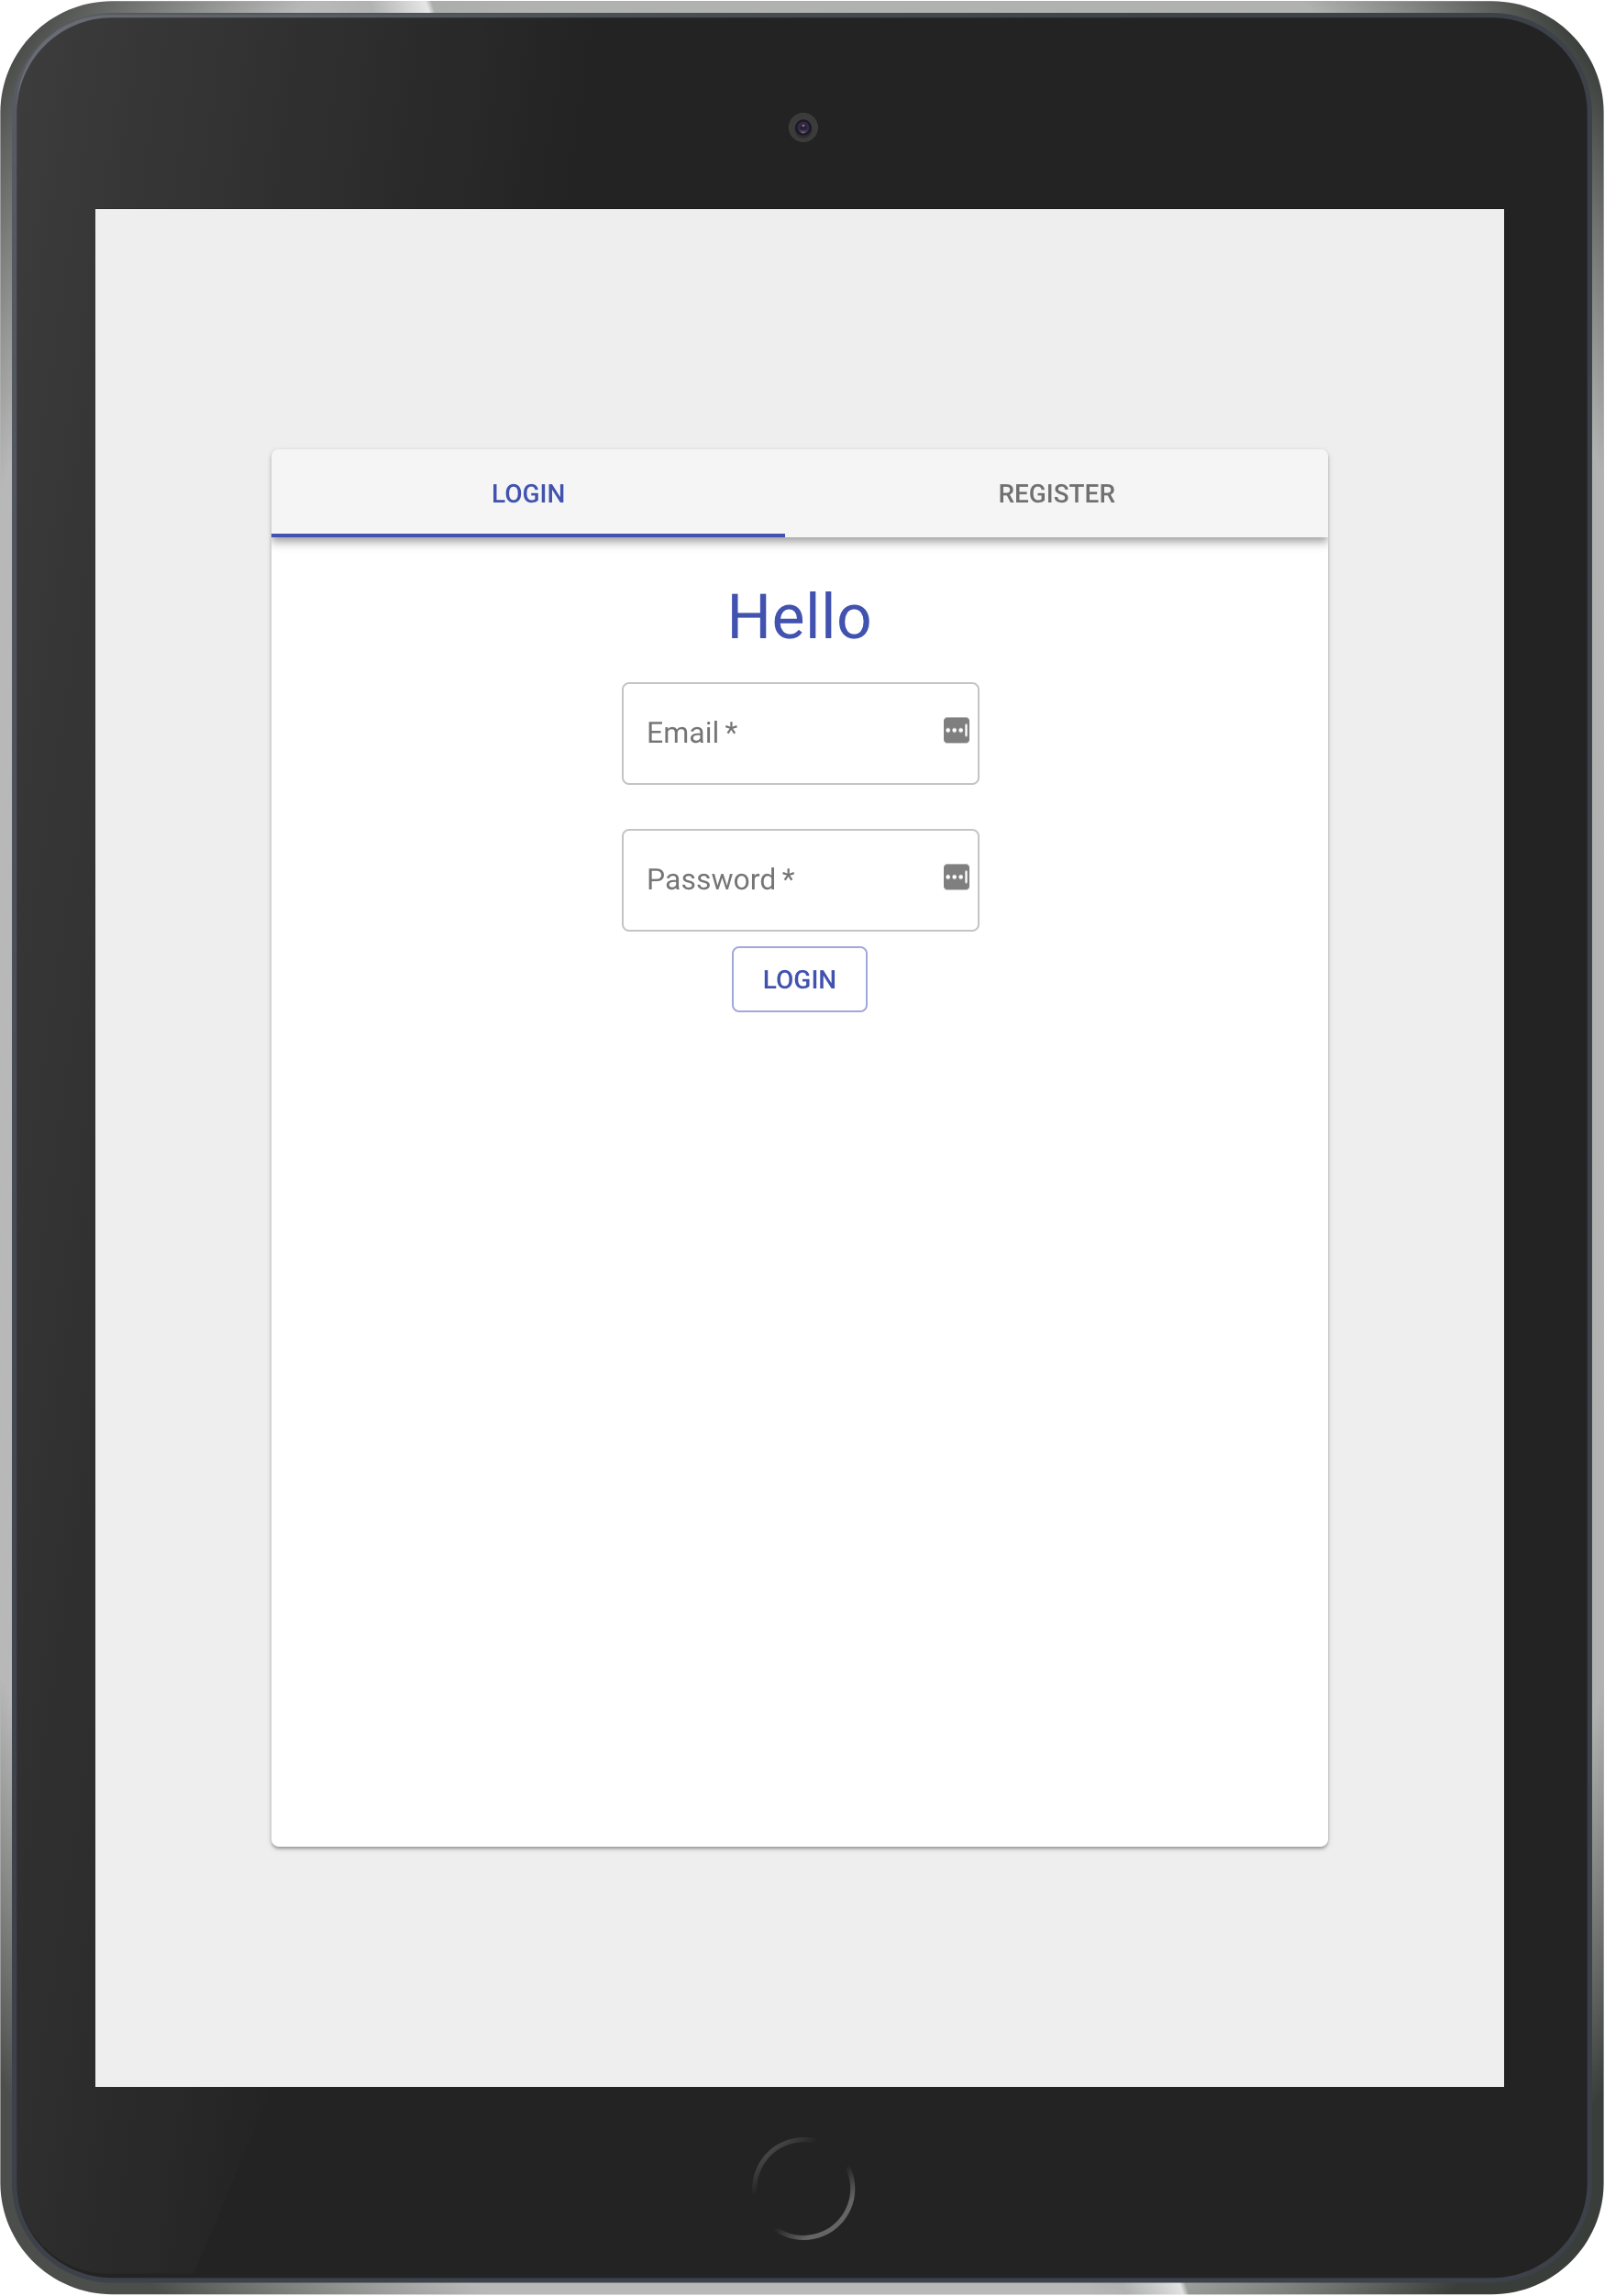
\includegraphics[width=5cm]{tablet_v_login.png}
 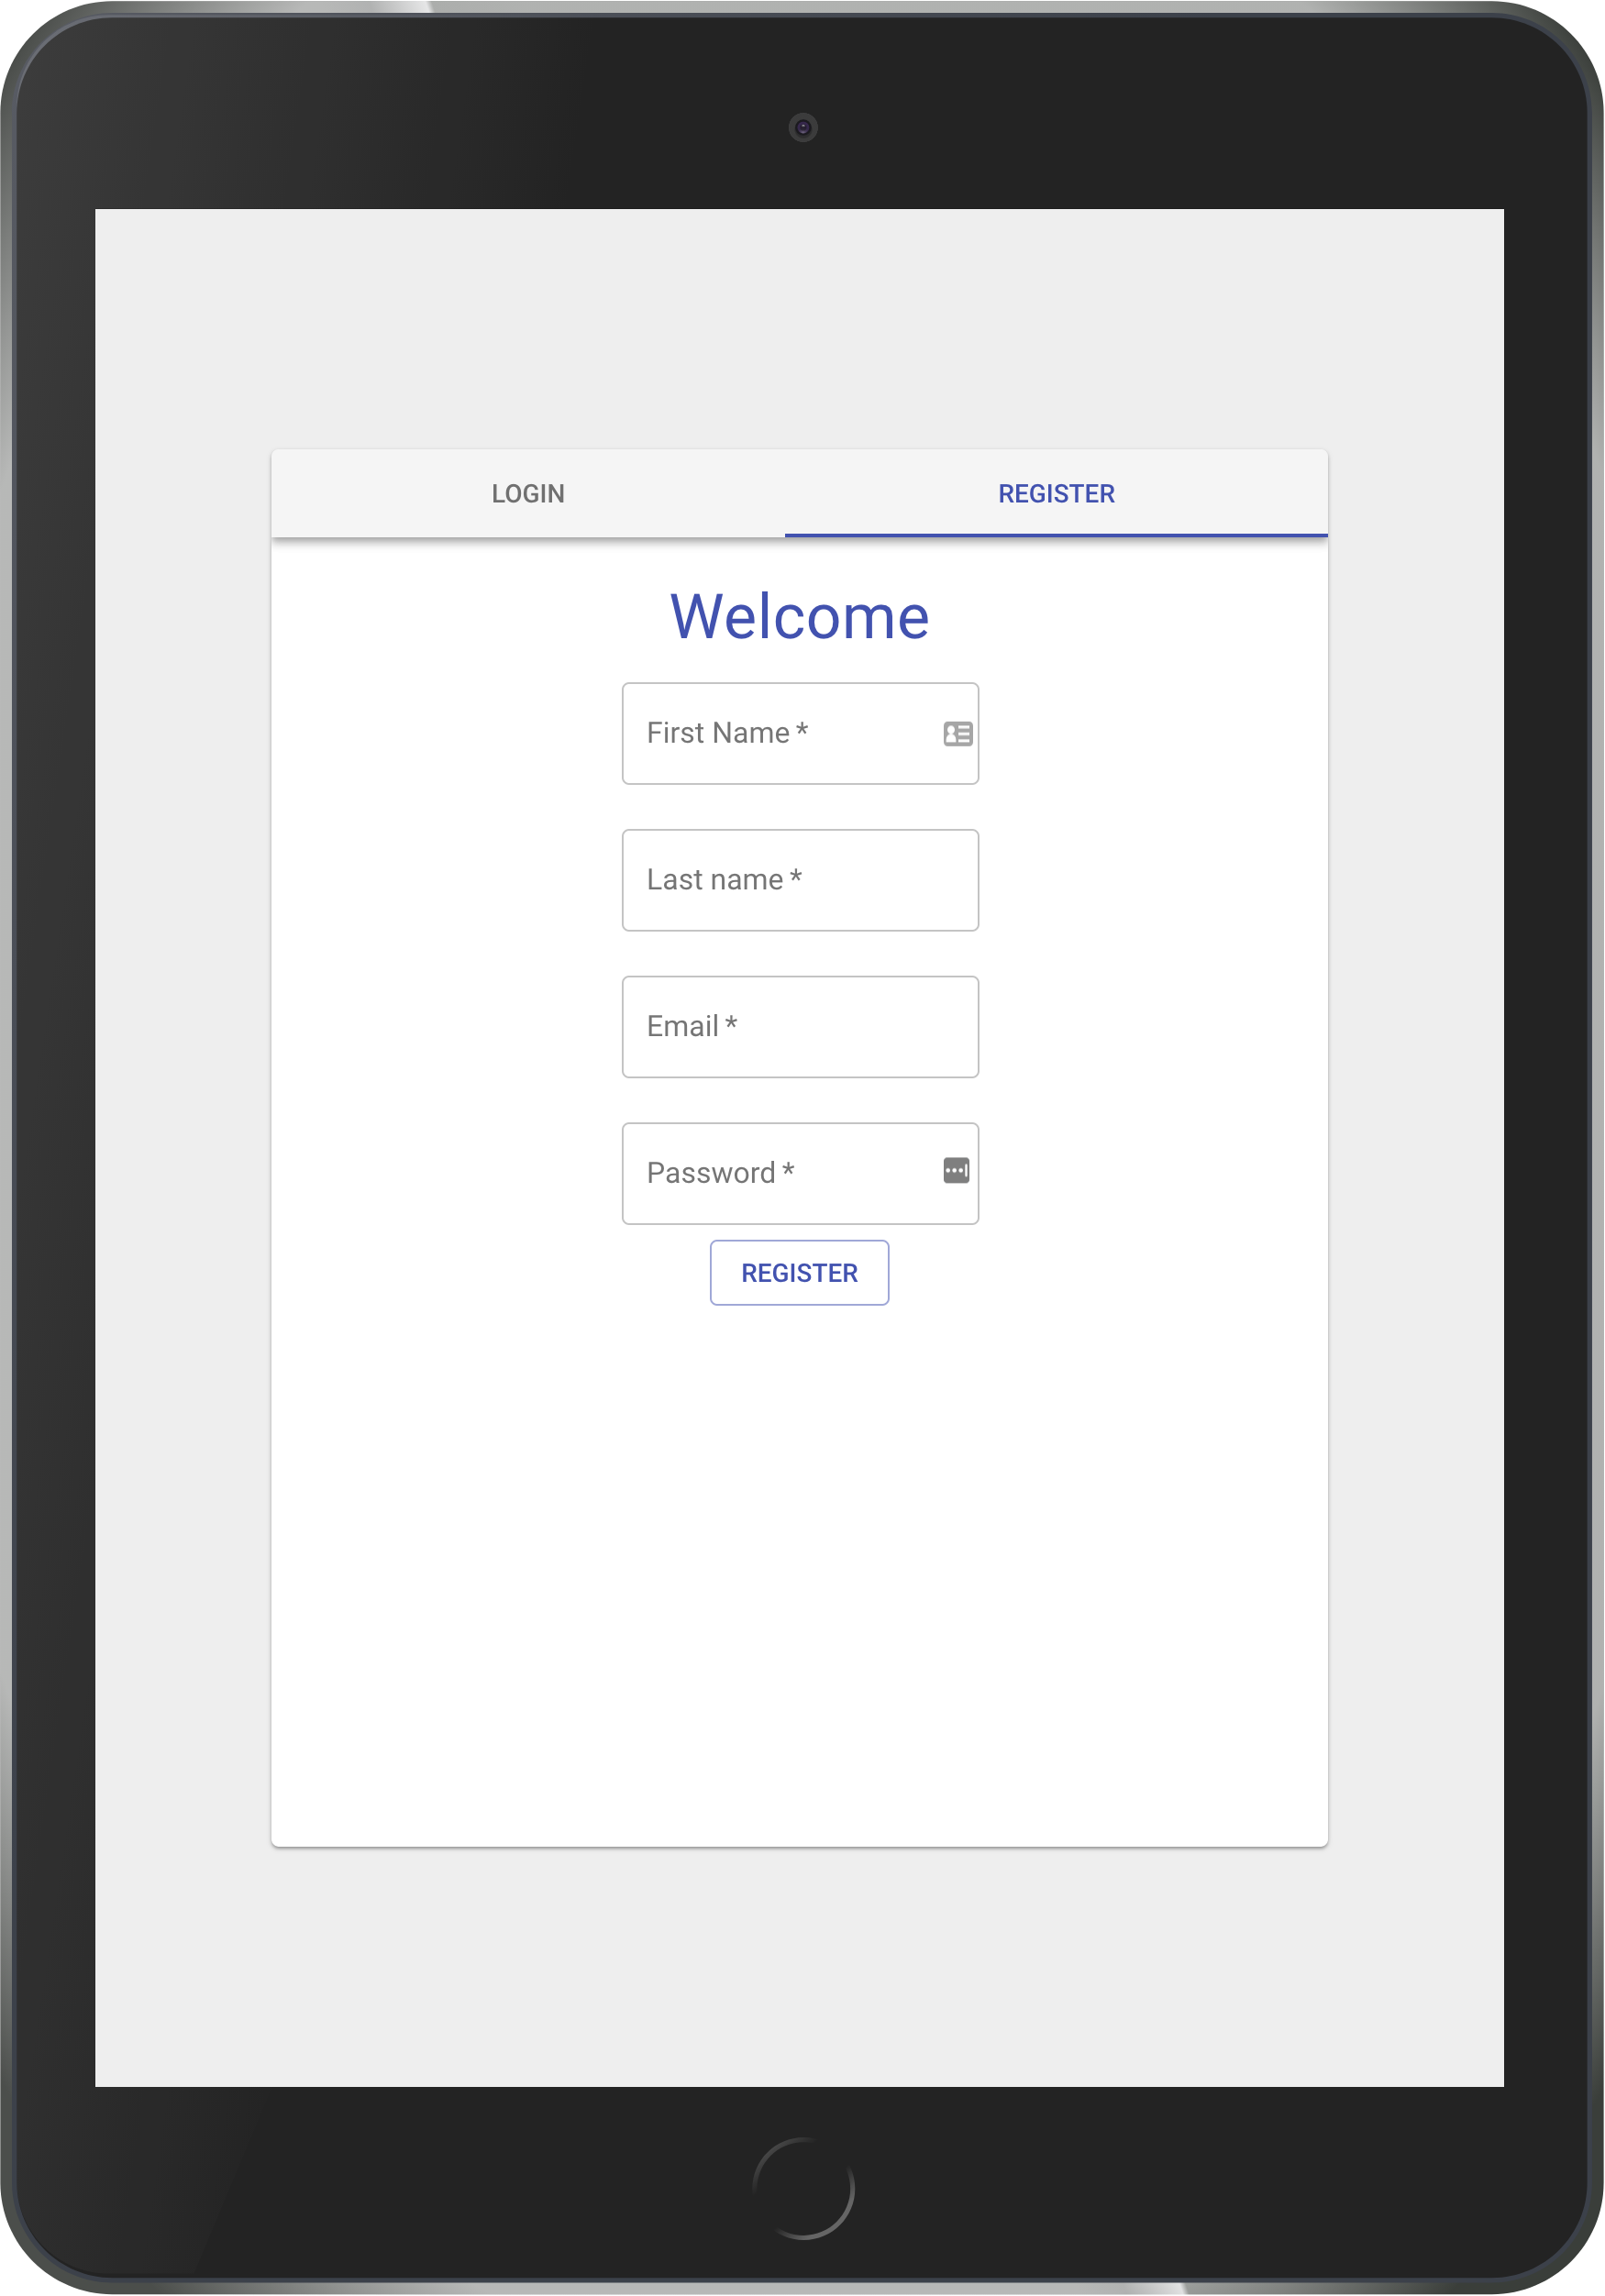
\includegraphics[width=5cm]{tablet_v_register.png}
 
 Tablet Horizontal:
 
 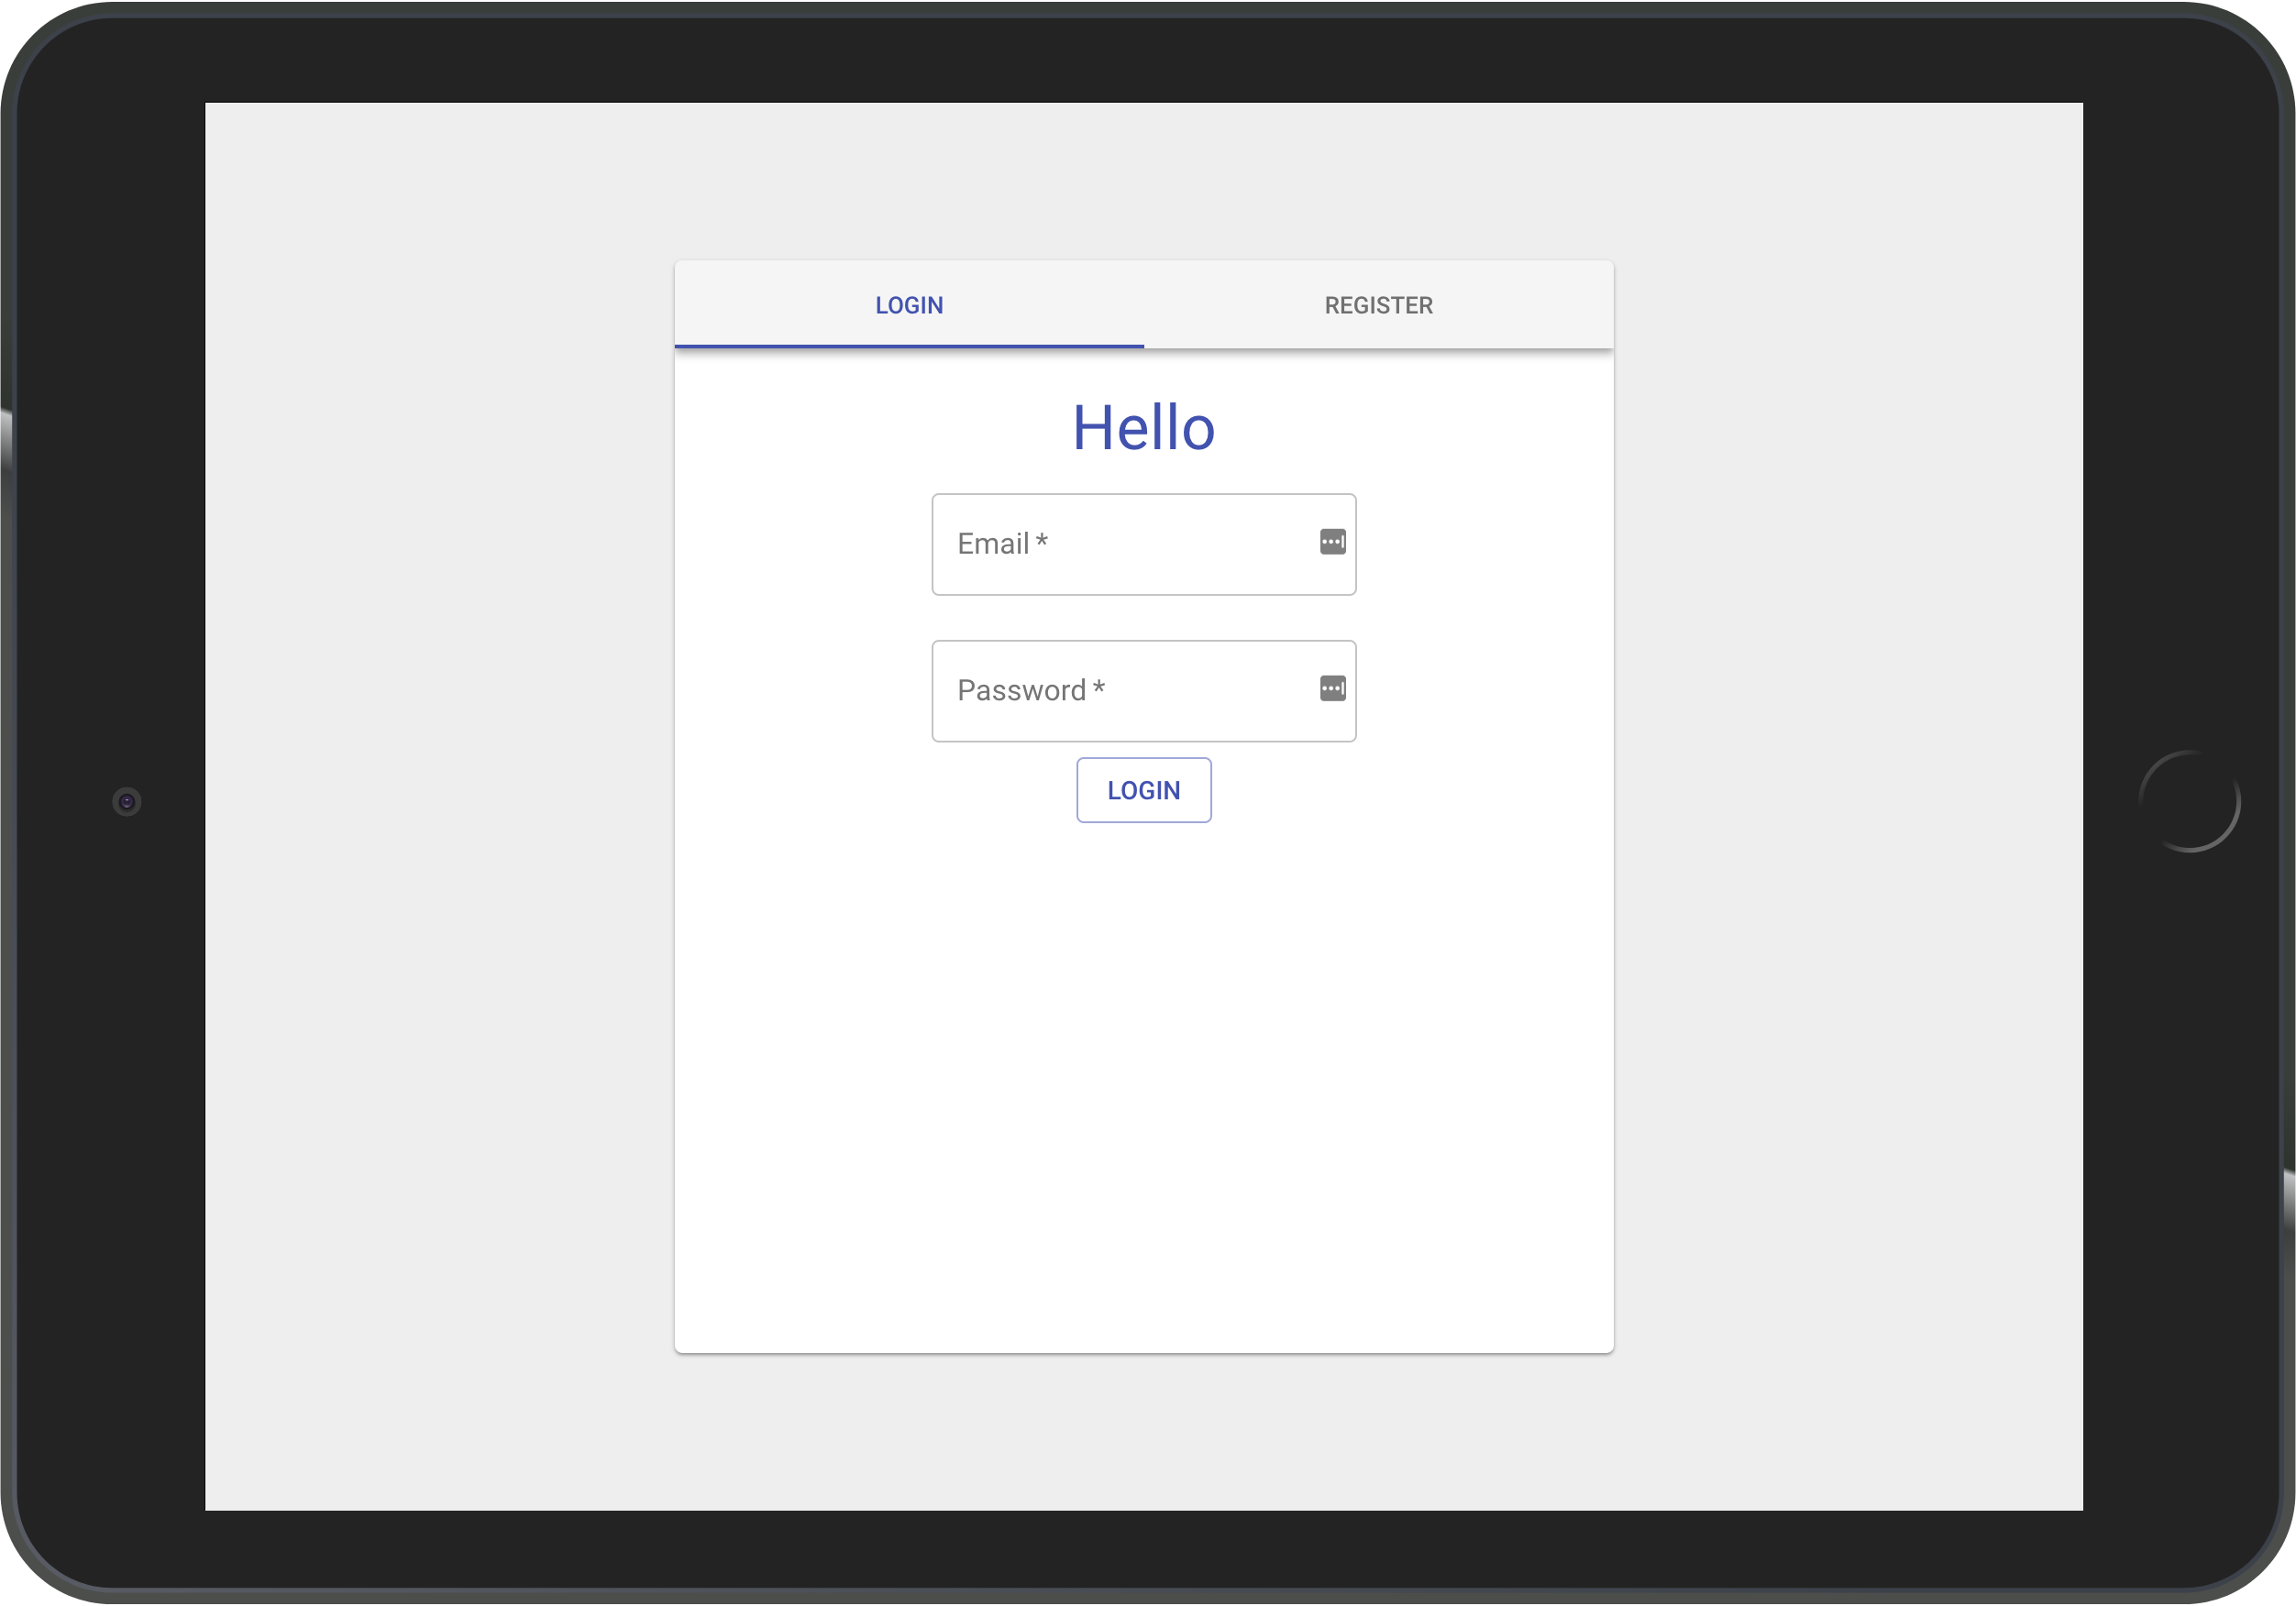
\includegraphics[width=6cm]{tablet_h_login.png}
 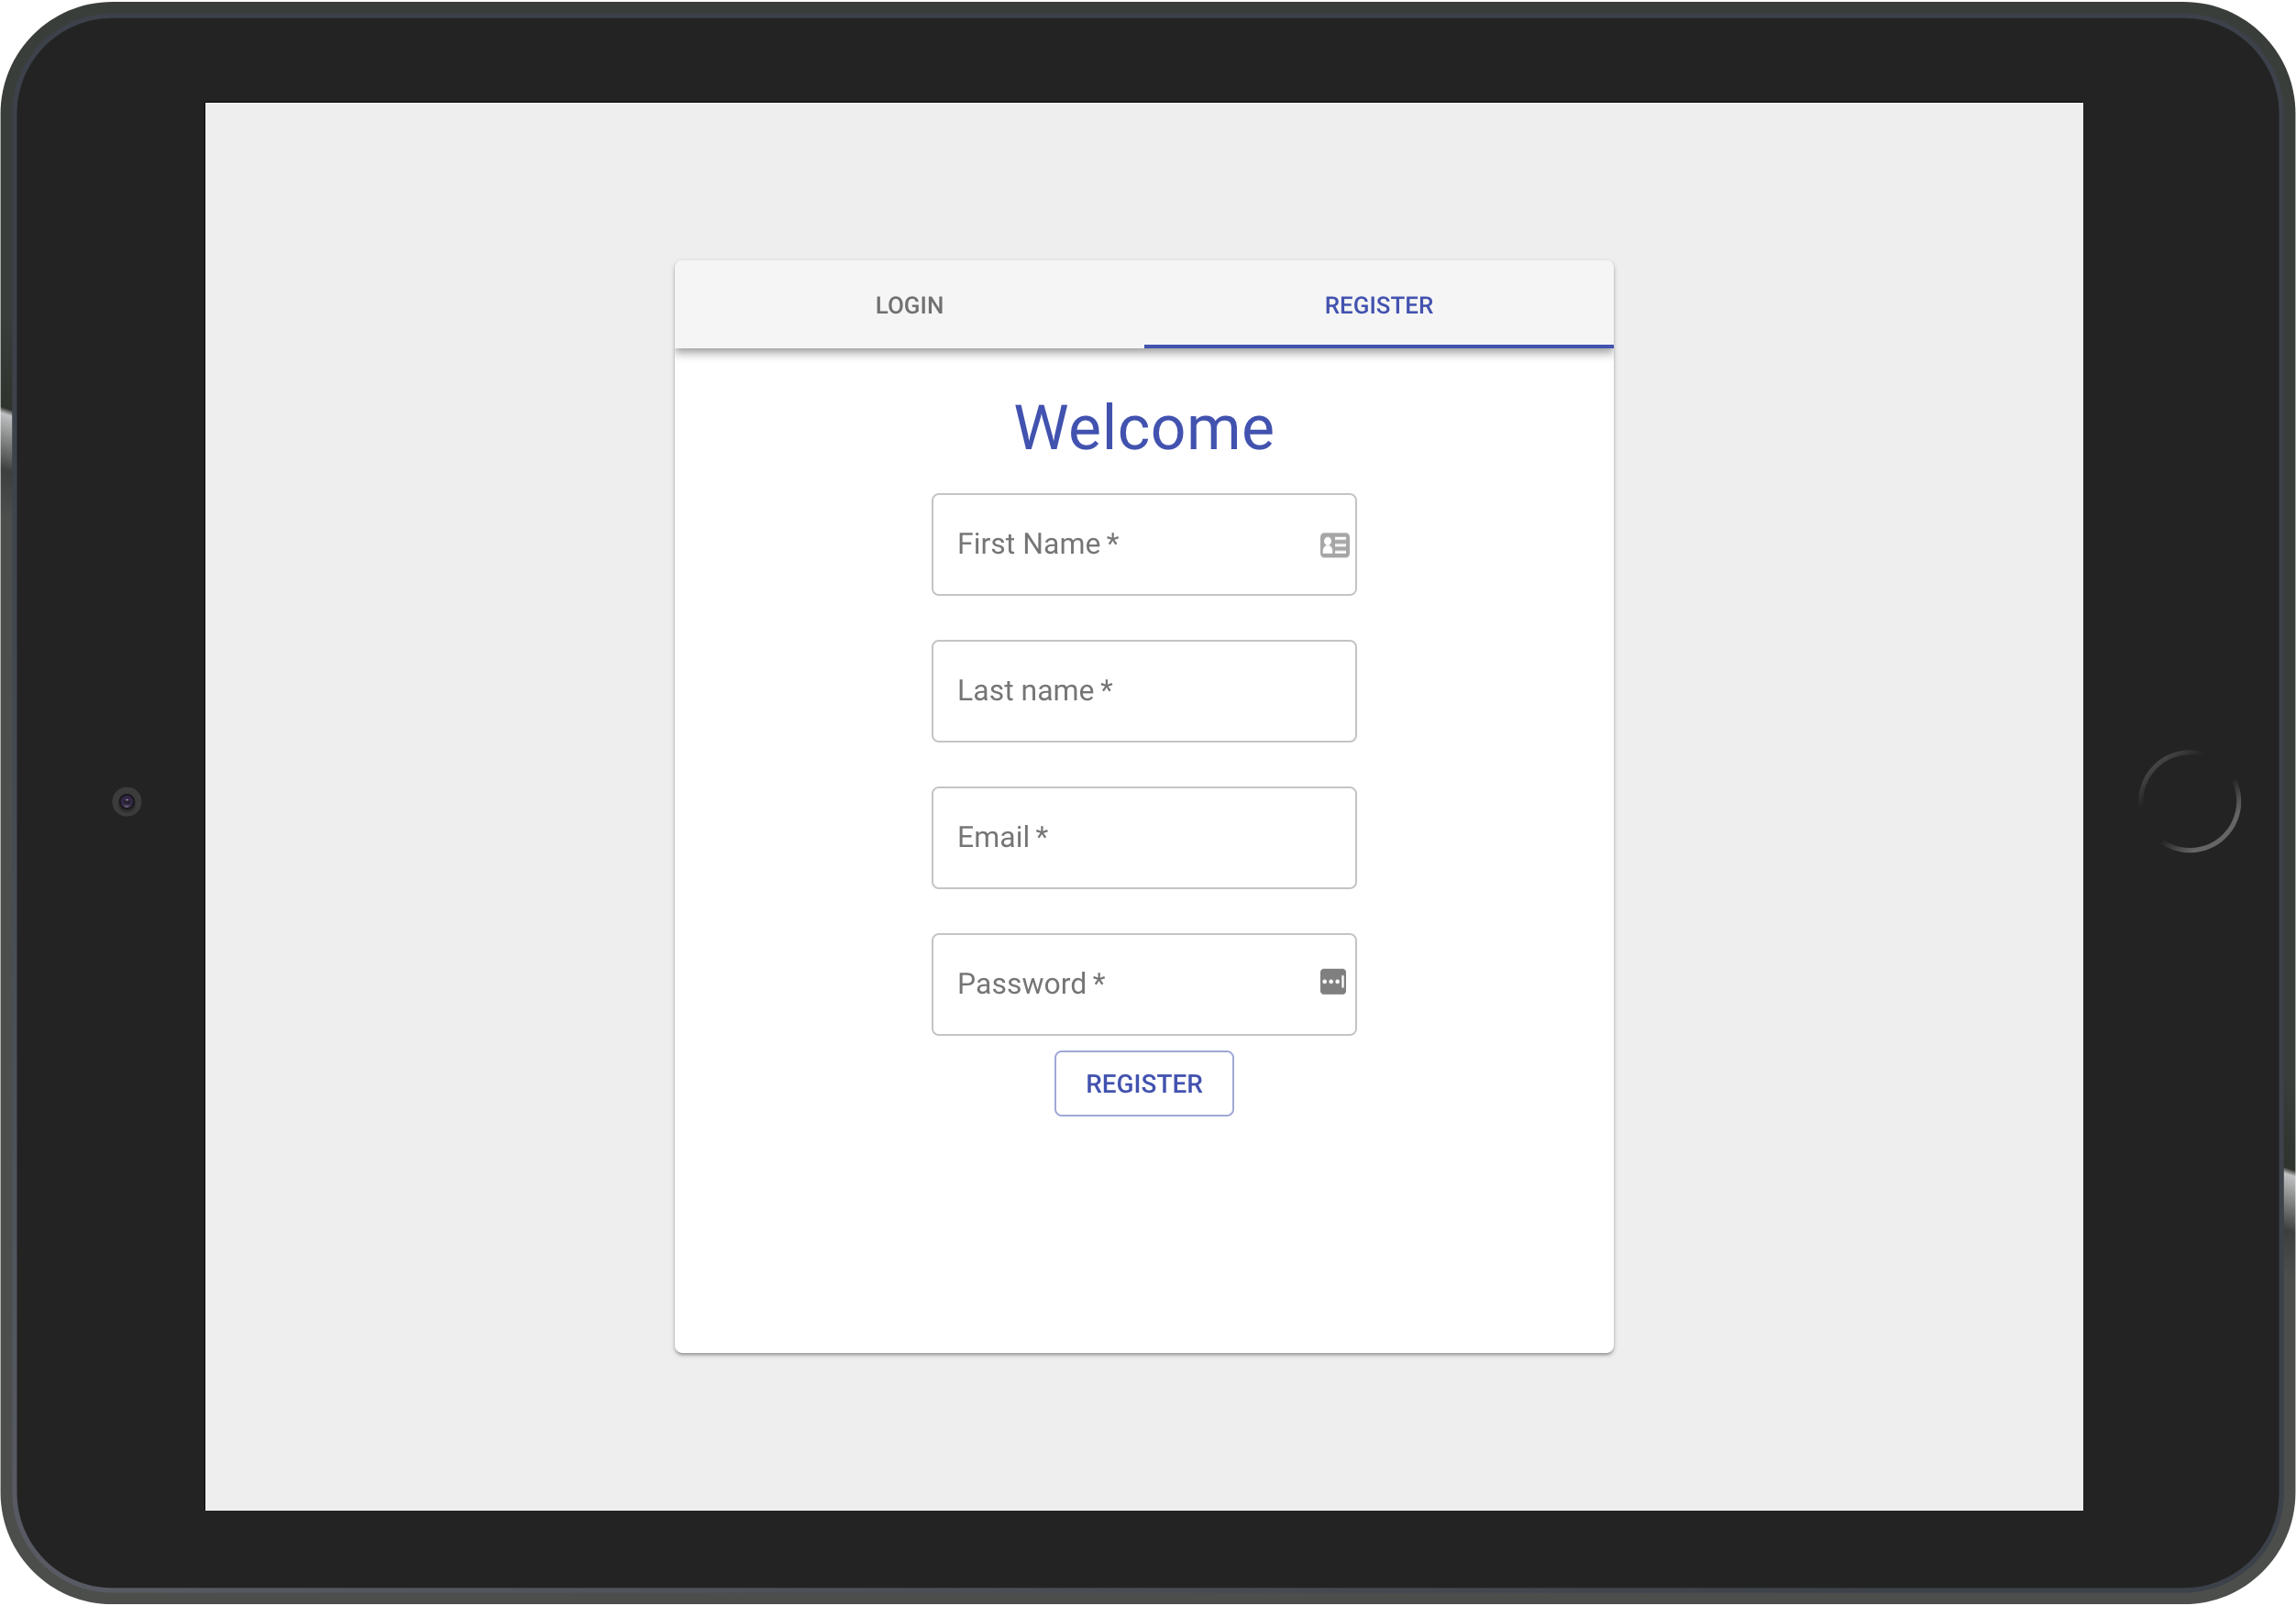
\includegraphics[width=6cm]{tablet_h_register.png}

  }
  \\
  \hline
\end{tabular}
\vskip 5mm

\begin{tabular}{|p{\colWidth}|}
	\hline
	\cellcolor{blue!25}\large
	\textbf{Include any quantitative data you have collected (this can be a graph/table with a few words)}
	\\ \hline
	\vtop to 200mm{
	\vspace{2mm}
	
Phone vertical:

 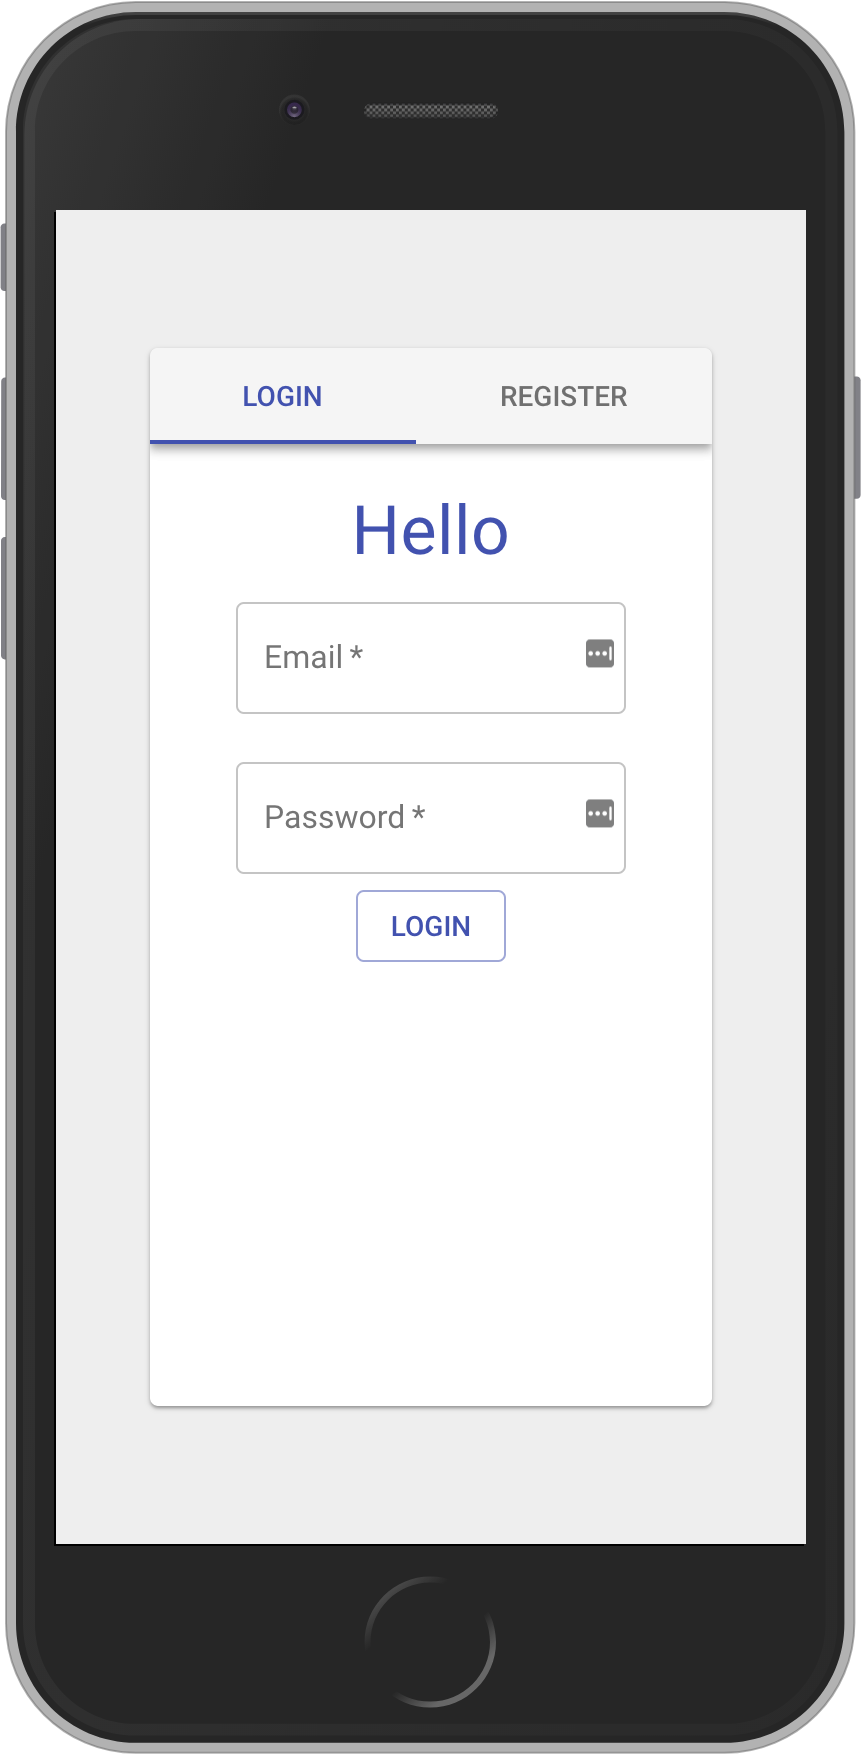
\includegraphics[width=4cm]{phone_v_login.png}
 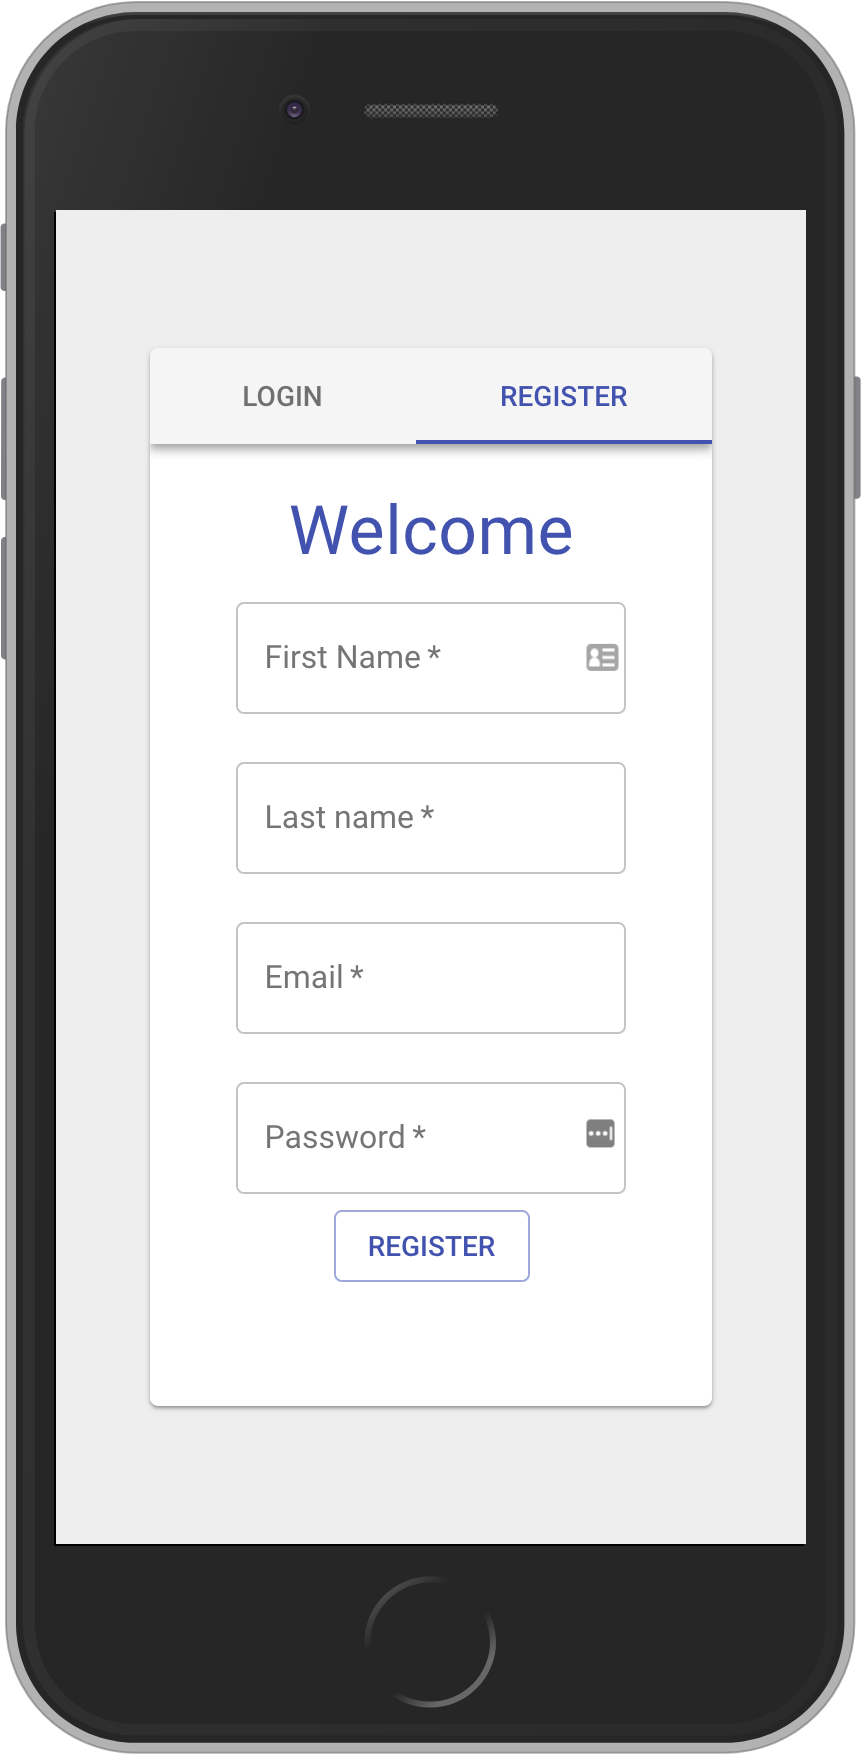
\includegraphics[width=4cm]{phone_v_register.png}
 

Phone horizontal:

 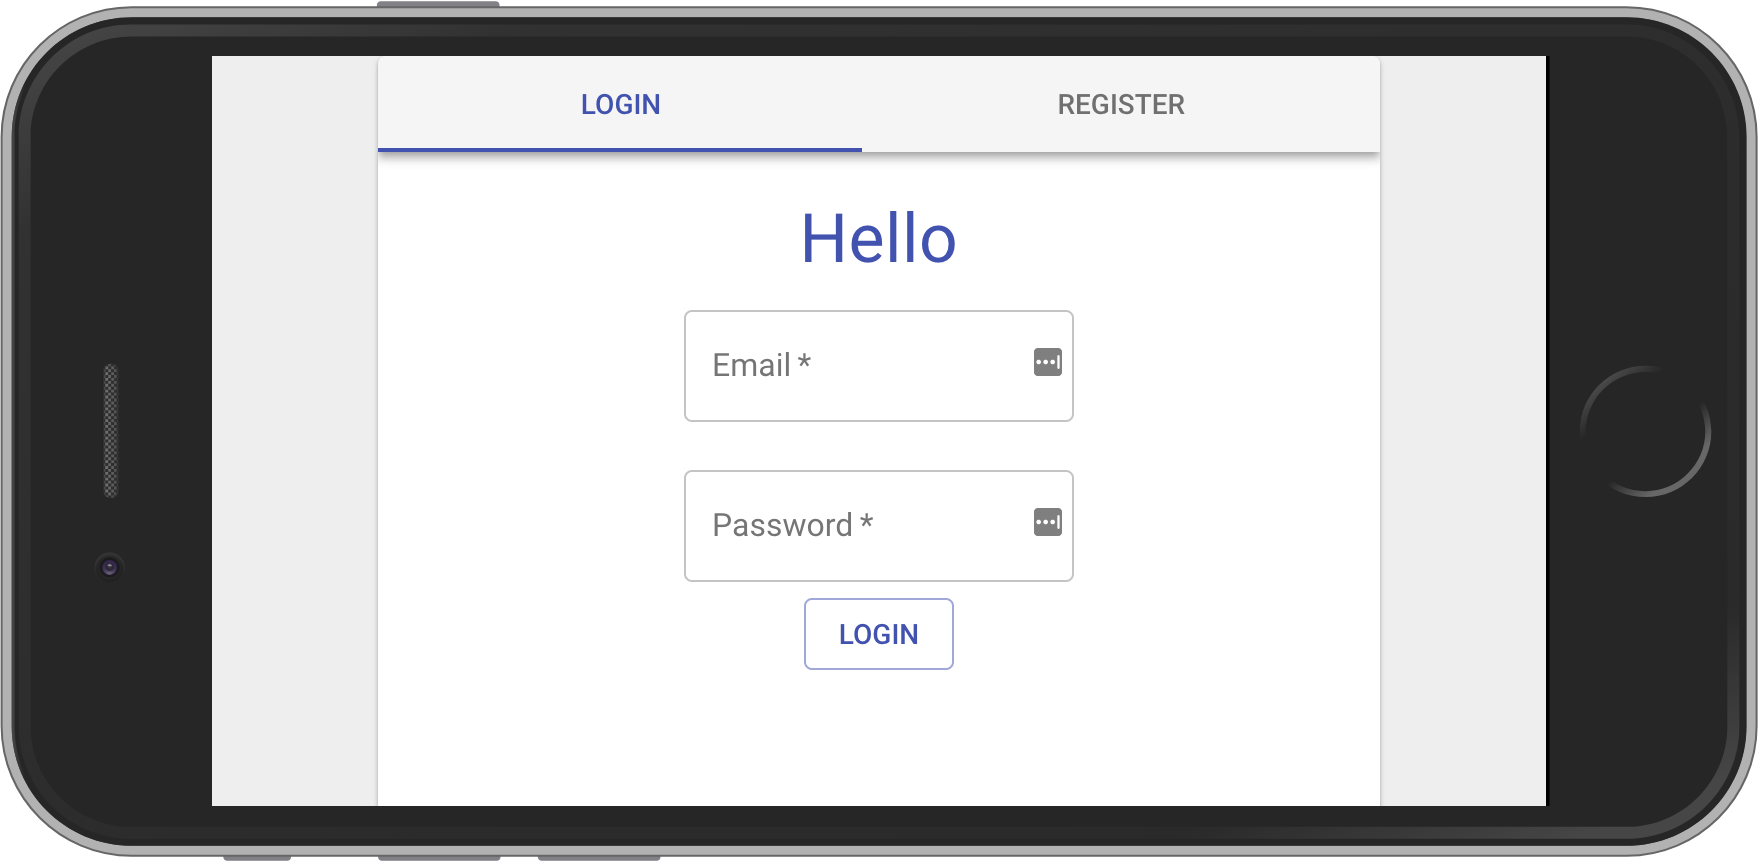
\includegraphics[width=6cm]{phone_h_login.png}
 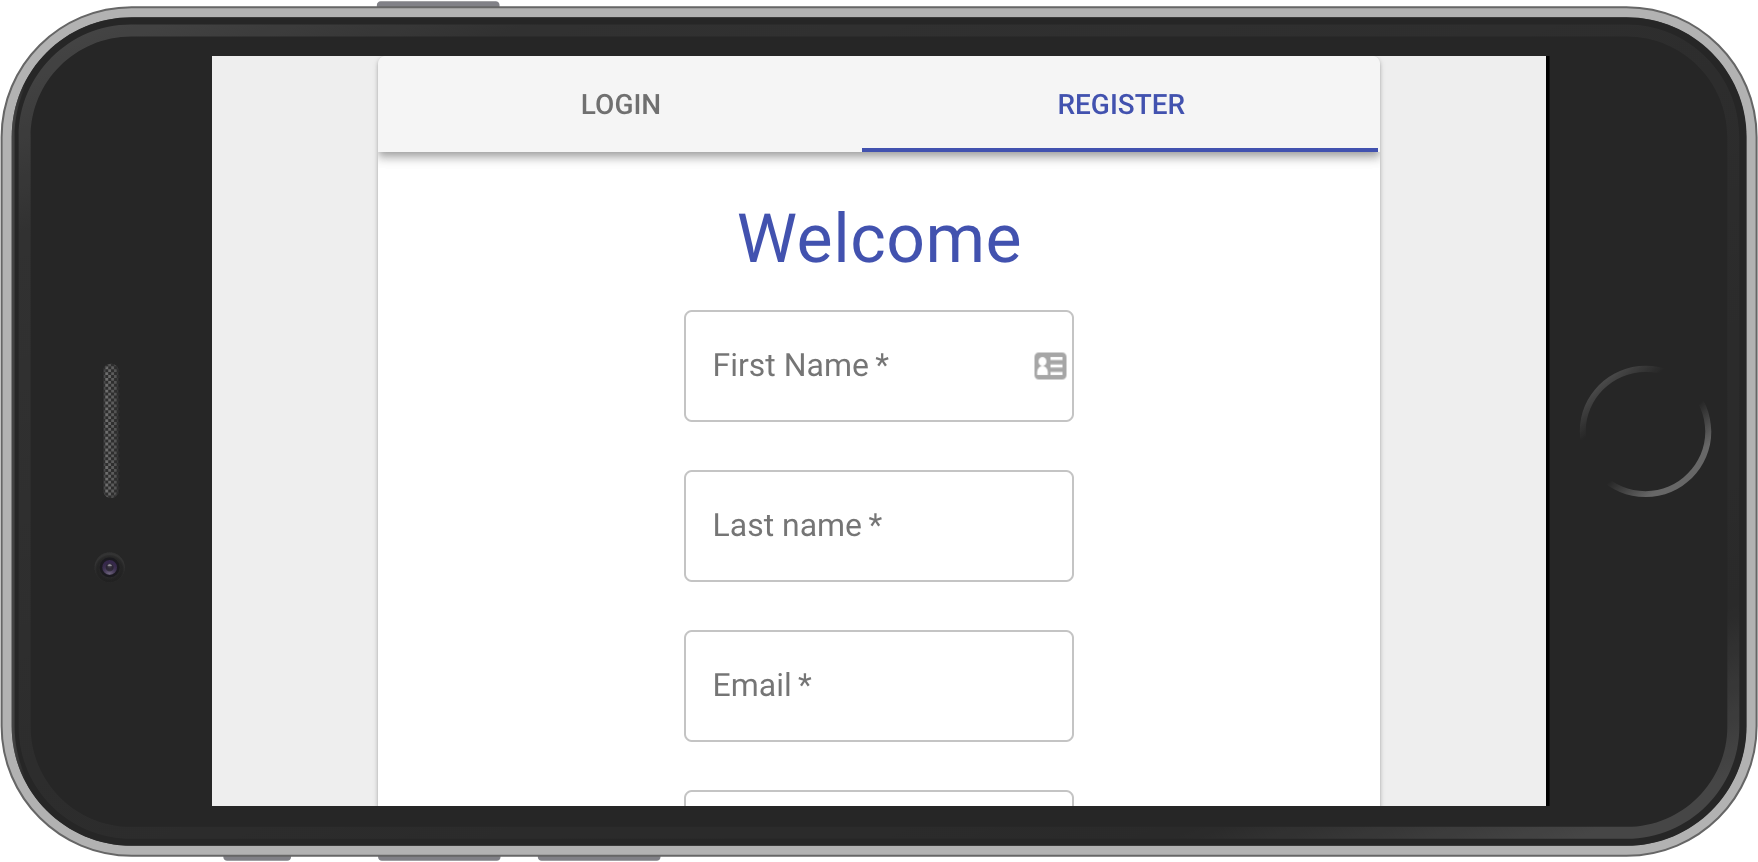
\includegraphics[width=6cm]{phone_h_register.png}

  }
  \\
  \hline
\end{tabular}
\vskip 5mm

% ------------NEXT STEPS----------

\begin{tabular}{|p{\colWidth}|}
	\hline
	\cellcolor{blue!25}\large
	\textbf{Say briefly what changes you will make to your plan for the next demo.}
	\\ \hline
	\vtop to 45mm{
We will divide the tasks more clearly between each sub-team, making the distinction between who is responsible for the robotics hardware and the robotics software. We also need to ensure better quality checking so that we are confident that when we have finished a part of the system, we can be sure that it will function as intended.We will also aim to have a finalised core robot design so we can design and print our food containers if necessary.
  \\
  \hline
\end{tabular}

\end{center}
  
\end{document}